\section{Case study: multitrait GWAS of 41 growth traits in \emph{Saccharomyces cerevisiae}}
Things to elaborate on further:
\begin{itemize}
\item missing data and imputation: MAR, NMAR; One crucial parameter in the imputation strategy are the number of predictor variables one choses for the imputation of a given target variable. As a general rule, using every bit of available information yields multiple imputations that have minimal bias and maximal certainty (Meng 1995; Collins et al. 2001). This principle implies that the number of predictors should be chosen as large as possible. Including as many predictors as possible tends to make the MAR assumption more plausible, thus reducing the need to make special adjustments for NMAR mechanisms (Schafer 1997).
\item 'multivariate imputations by chained equations (MICE) \citep{vanBuuren2011}, which generates imputations for incomplete multivariate data by Gibbs sampling.
\item The imputation itself was done by predictive mean matching (PMM) \citep{Little1988}. PMM is a semi-parametric imputation method which can preserve non-linear relations in the data. 
\item multiple testing correction: Bonferroni, Benjamini and Hochberg, effective number of tests
\end{itemize}
The yeast dataset from a study by Bloom and colleagues \citeyearpar{Bloom2013} is used as case study dataset to show the feasibility of LiMMBo.

\subsection{Data}
\paragraph{Public dataset} The dataset consists of phenotype and genotype data of 1,008 prototrophic haploid \emph{Saccharomyces cerevisiae} segregants derived from a cross between a laboratory strain and a wine strain strains. It contains 11,623 unique genotypic markers obtained via short-read sequencing for all 1,008 segregants (no missing genotypes). For phenotyping, they grew segregants on agar plates under 46 different conditions, including different temperatures, pH and nutrient addition (see labels in Figure~\ref{fig:traitcorrelations}). The phenotypes were definded as end-point colony size normalized relative to growth on control medium. For the remainder of this chapter, a trait is defined as the normalised growth size in one conditions.
\paragraph{Phenotype imputation. } Out of the 1,008 segregants, 303 were phenotyped for all 46 traits. Missing phenotypes are not evenly distributed with some traits such as cobalt chloride being present for almost all samples and others such as sorbitol or raffinose are lacking in more than a third of the samples. The distribution of trait missingness across all samples is depicted in Figure~\ref{fig:missingness-all}. 

\begin{figure}[!h]
	\centering
	\begin{subfigure}[b]{0.48\textwidth}
		%\hspace{3cm}
		\center
	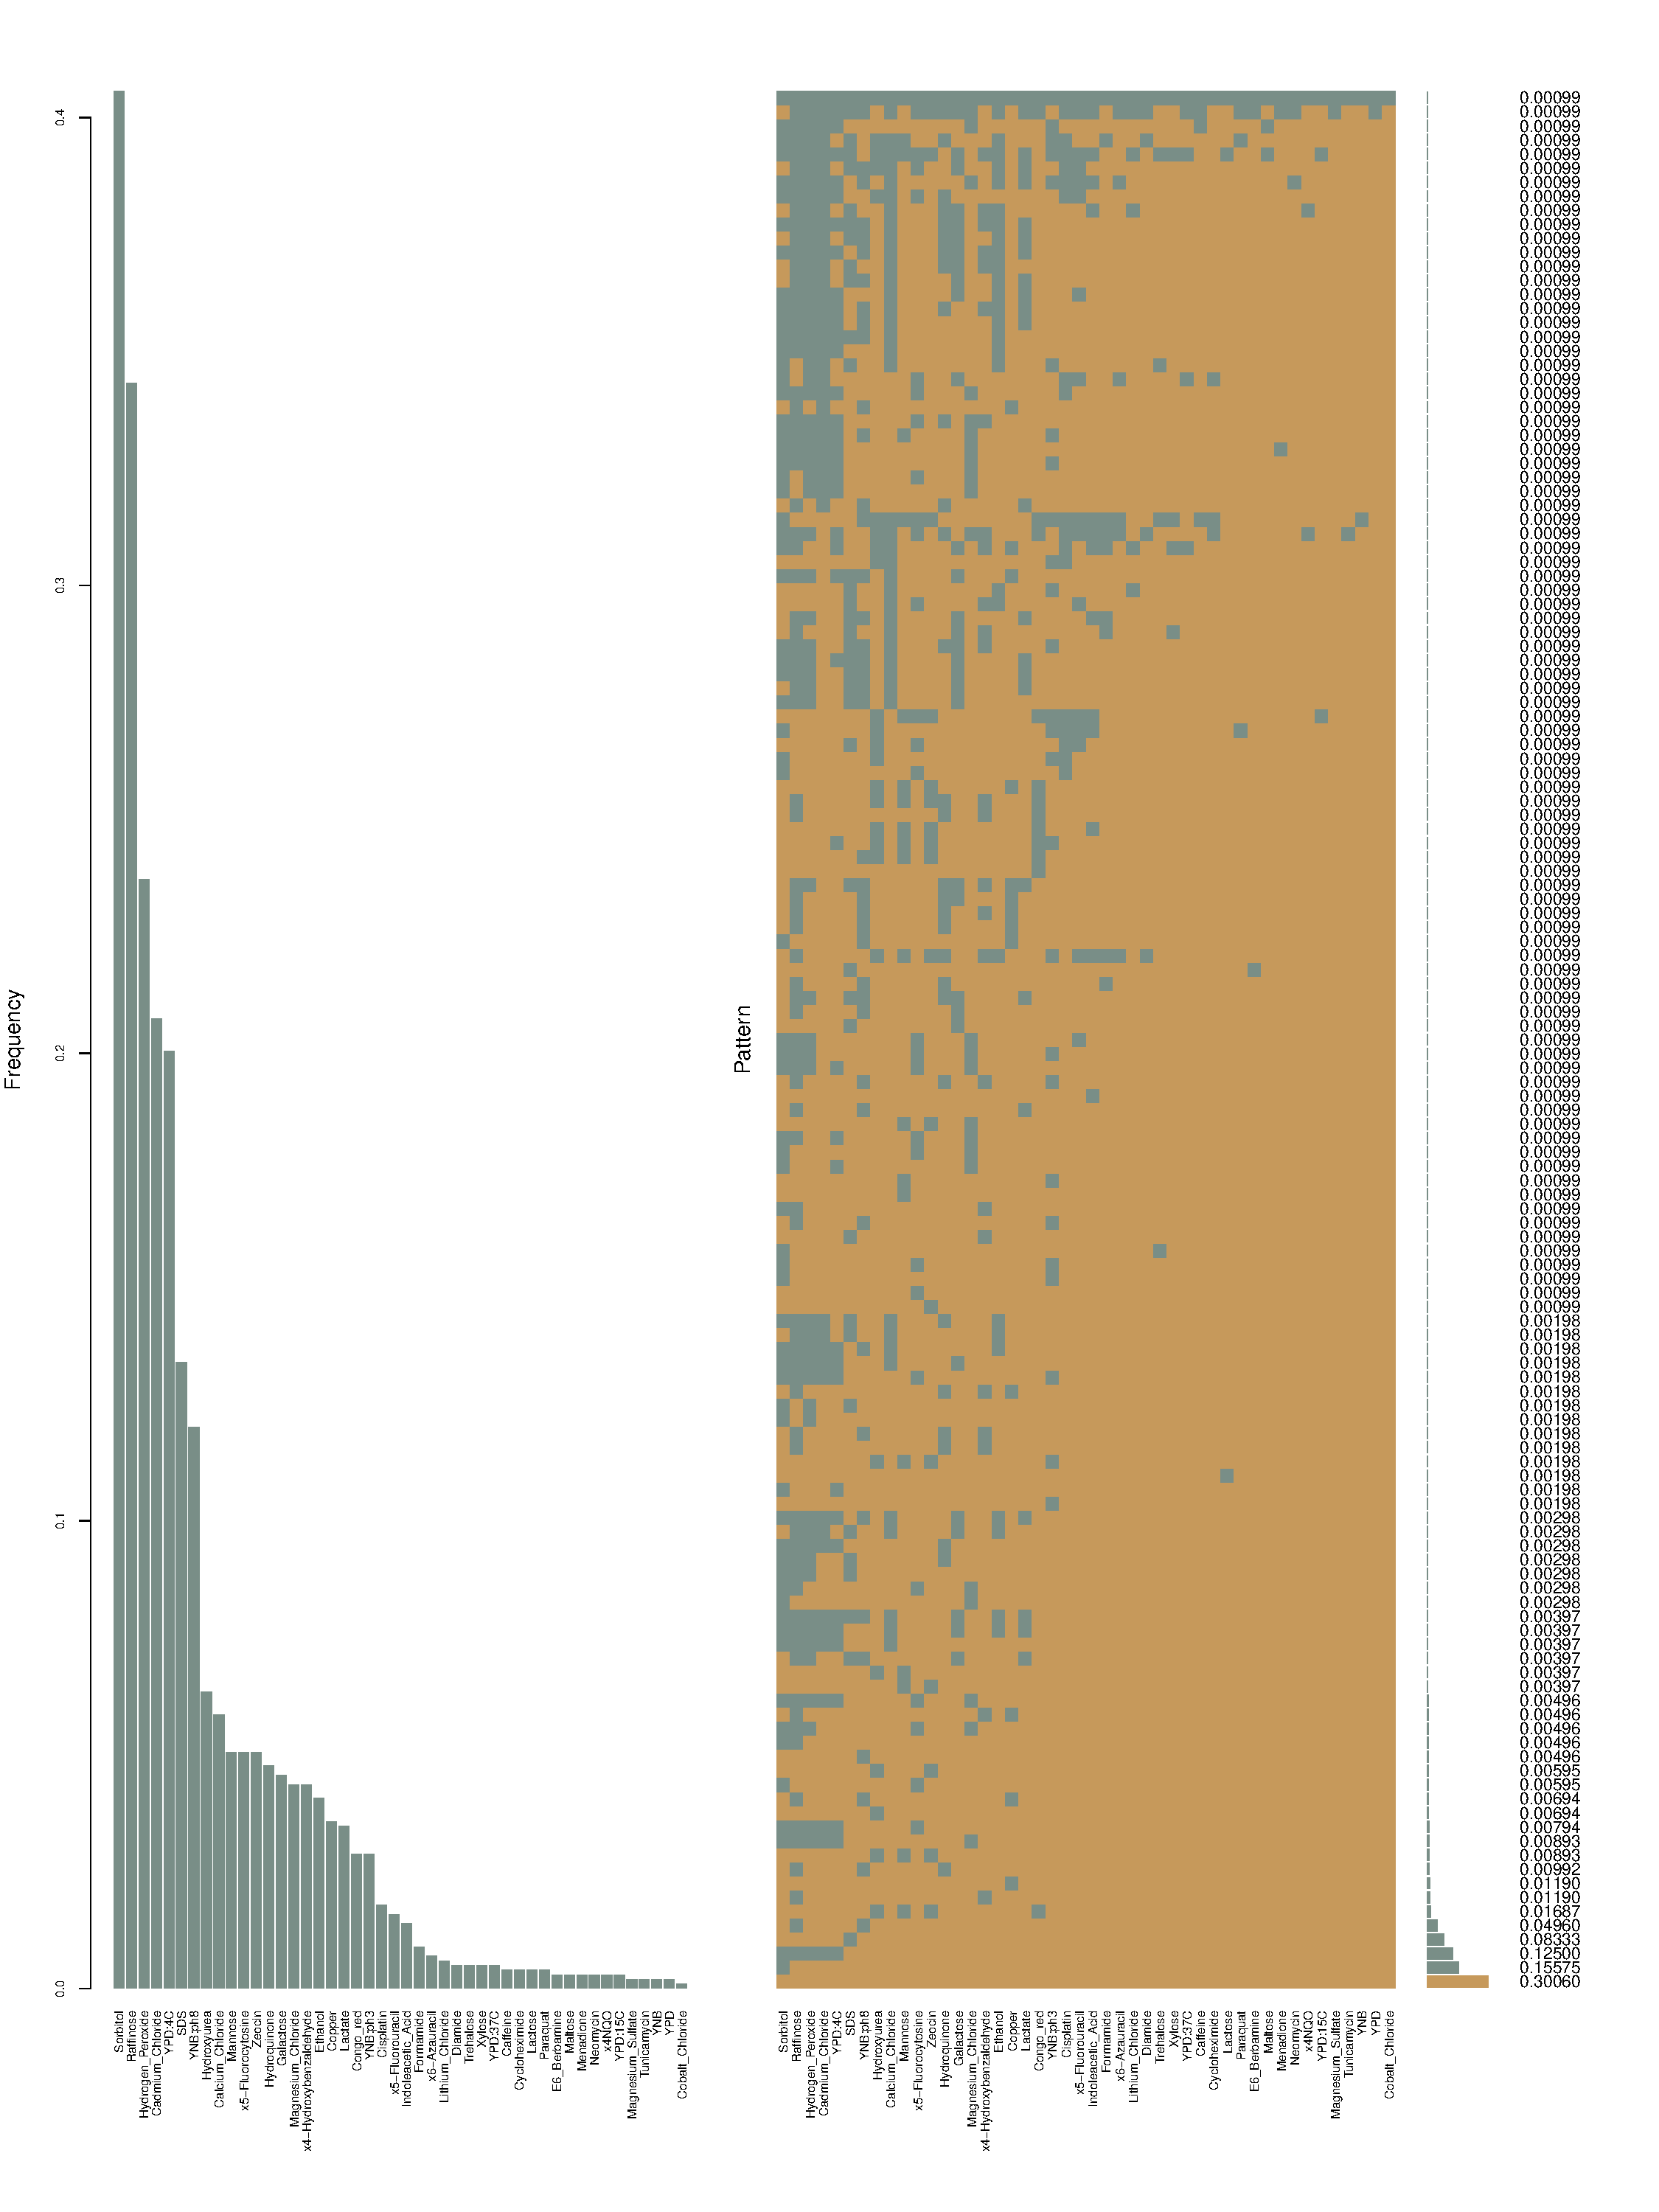
\includegraphics[trim = 0mm 0mm 20mm 2mm, clip, scale=0.2]{Chapter1/Figures/20170124_missing_data_pattern.pdf}
	\caption{\textbf{Full dataset}}
 		\label{fig:missingness-all}
	\end{subfigure}
	~
	\begin{subfigure}[b]{0.48\textwidth}
		%\hspace{3cm}
		\center
	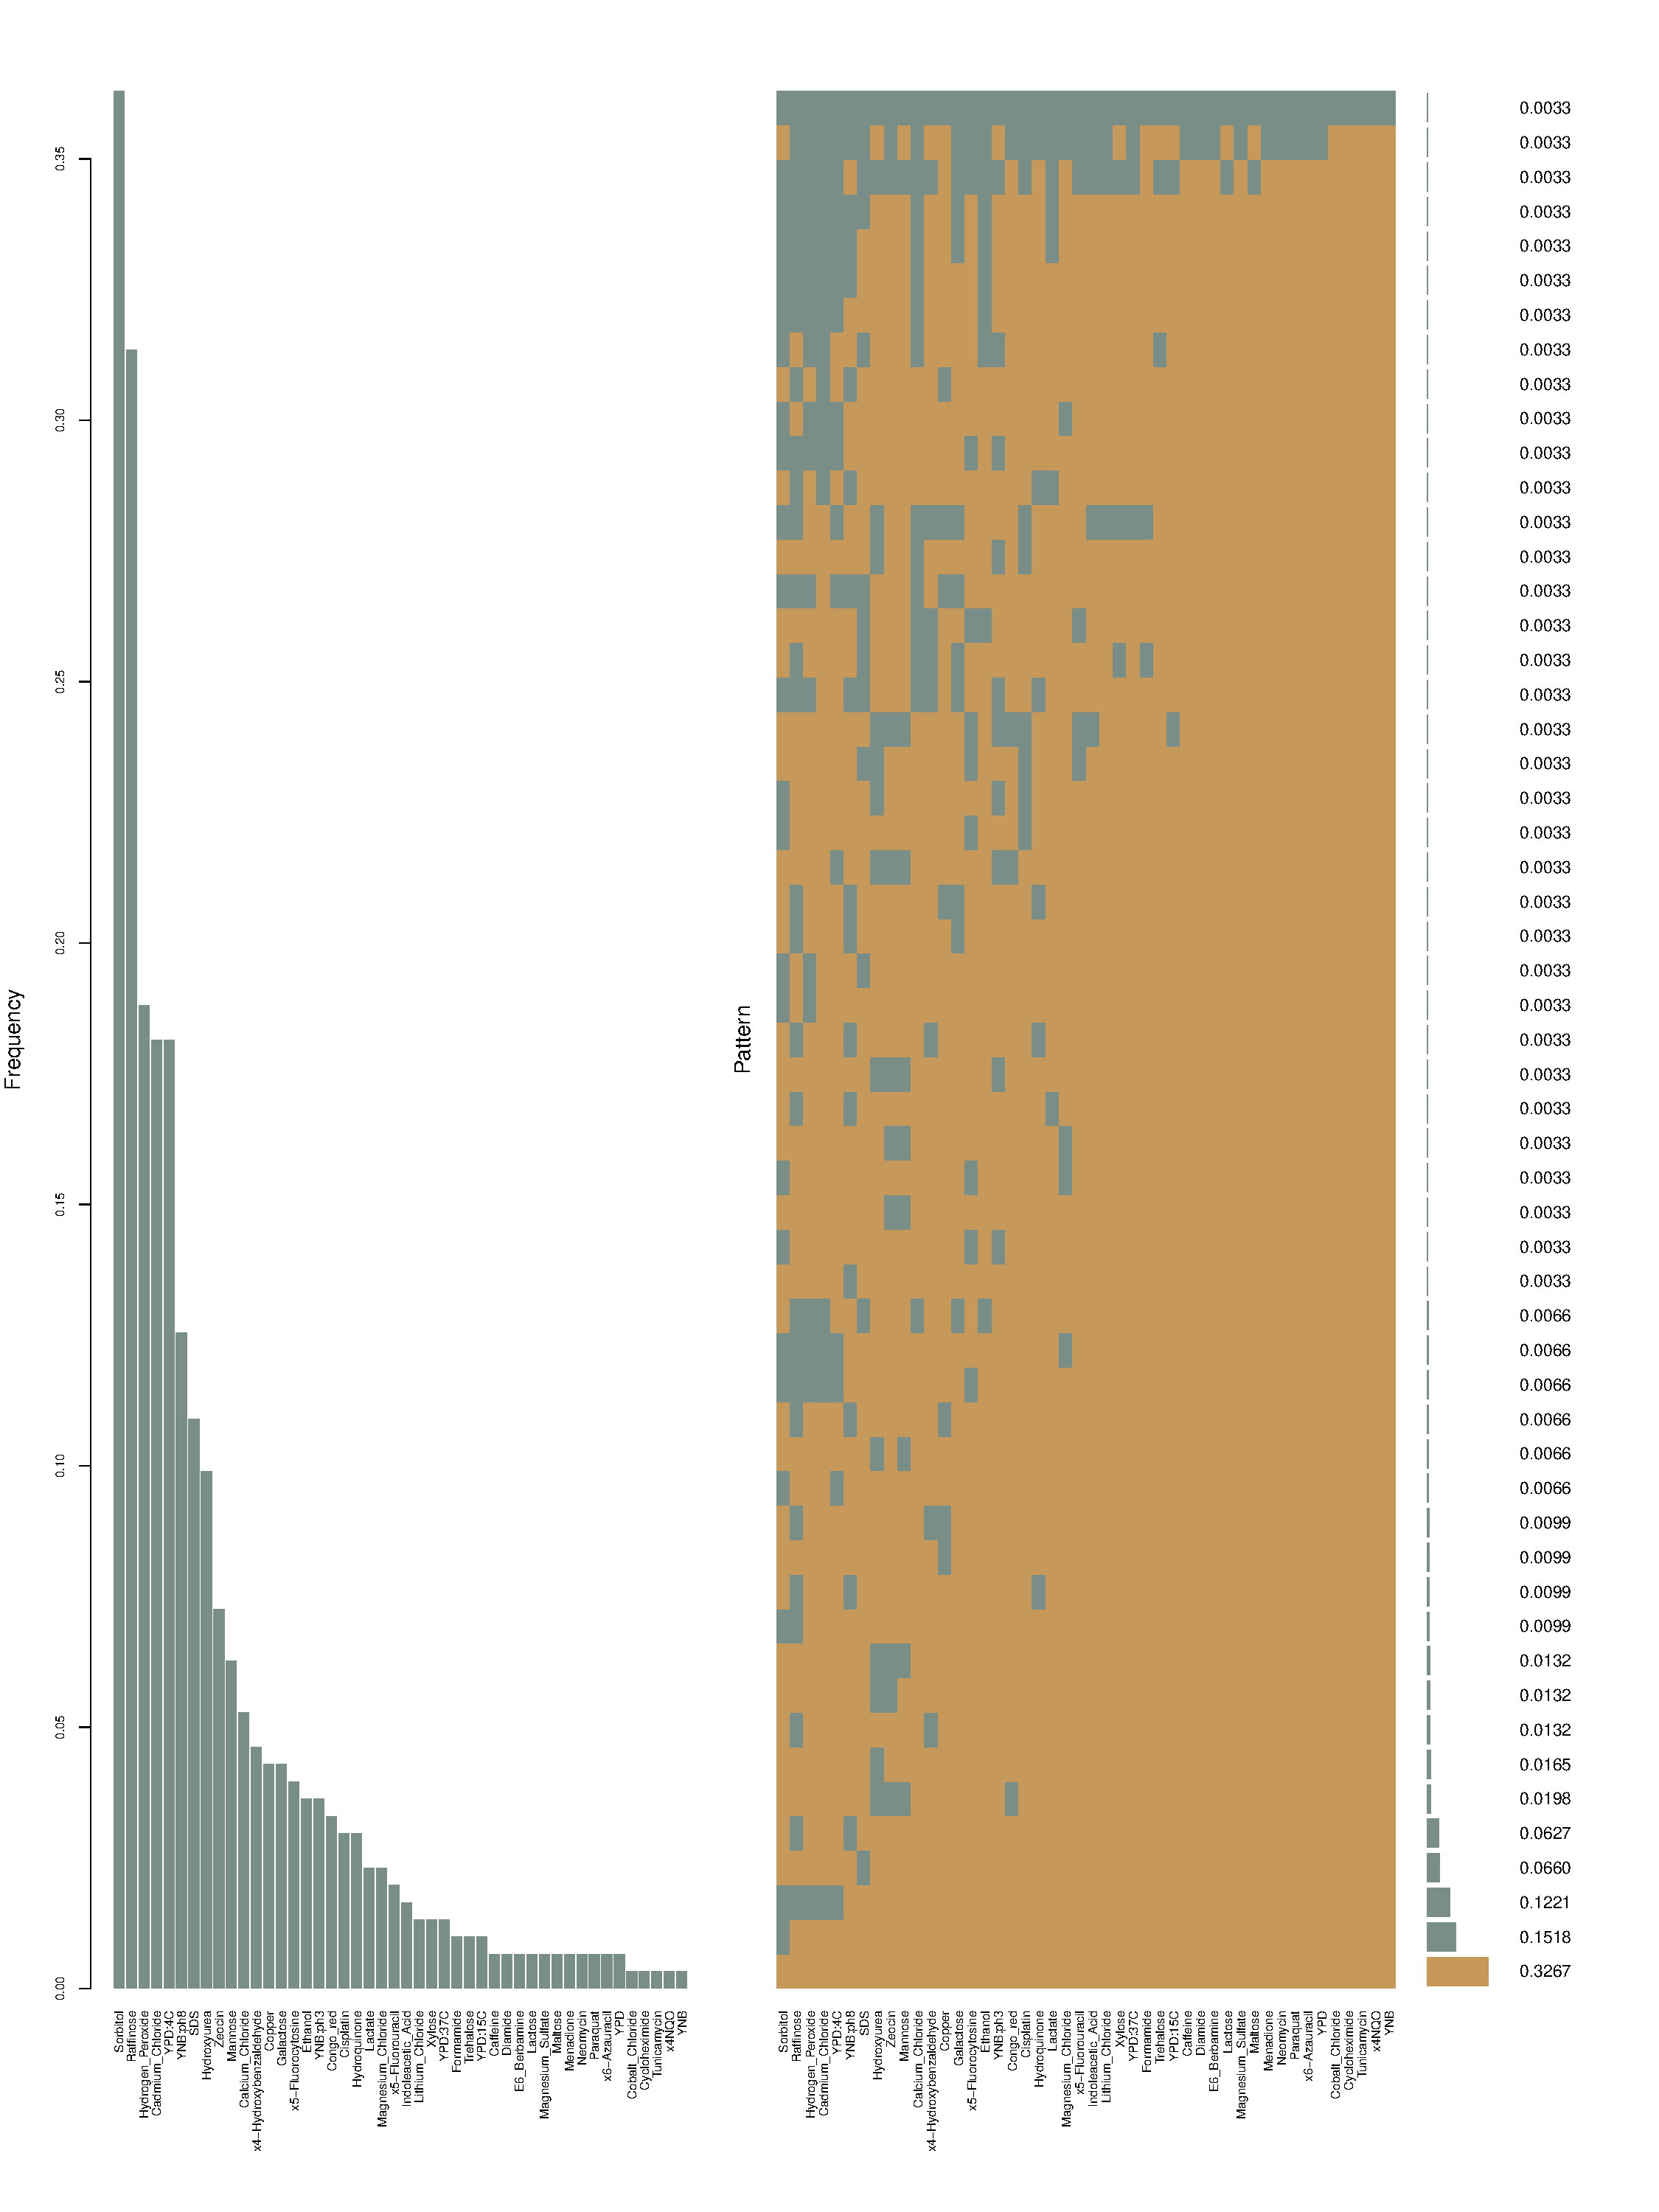
\includegraphics[trim = 0mm 0mm 20mm 2mm, clip, scale=0.2]{Chapter1/Figures/20170124_missing_data_pattern_simulated.pdf}\\
	\caption{\textbf{Simulated  dataset}}
 		\label{fig:missingness-sample}
	\end{subfigure}
	\caption[Frequencies and distributions of missing values in the yeast phenotype data]{\textbf{Frequencies and distributions of missing values in the yeast phenotype data.} In both panels, the histogram (left) shows the frequency of missing values for a particular trait. The aggregation plot (middle) depicts all existing combinations of missing and non-missing values in the traits. The bar chart and numbers (right) show the frequencies of occurrence of the different combinations (R Package: \emph{VIM} \citep{Templ2012}). (a) The full dataset contains normalised colony sizes for growth in 46 different conditions of 1,008 genotyped yeast segregants as derived from \citep{Bloom2013}. 306 segregants are fully genotyped (bar chart, orange bar). (b) Fully-phenotyped dataset of 306 segreagants with simulated missing values based on missingness patterns for then entire pool of 1,008 segregants.}
 	\label{fig:missingness}
\end{figure}

The LMM framework relies on all samples being fully genotyped and phenotyped and does not accept missing values. In order to use the largest possible subset of the data, I investigated imputation strategies for the missing phenotypes. I used the subset of 303 fully phenotyped samples to determine traits suitable for imputation. I simulated data with a similar pattern of missingness as observed in the original dataset by subsampling the full dataset to the subset size and overlaying the observed missingness pattern onto the subset of 303 fully phenotyped samples. The resulting pattern is depicted in Figure~\ref{fig:missingness-sample}. Similar results in frequencies of fully phenotyped samples and combination of missing/non-missing traits can be observed when comparing it to the original frequencies and patterns (Figure~\ref{fig:missingness-all}). I chose the MICE framework \citep{vanBuuren2011} with PMM as the imputation method to determine the most suitable imputation parameter settings in the simulated dataset which would then be applied to impute the real missing values in the full dataset. The predictor variables for each trait were determined based on its pair-wise Spearman's rank correlation coefficient \(\rho\) with all other traits in the dataset (Figure~\ref{fig:traitcorrelations}). In addition, only predictor traits that had been measured in at least 20\% of the samples in the dataset were considered. Different predictor variable set-ups were examined based on increasing thresholds for the Spearman's Rank correlation coefficient: \(\rho =\left\{0, 0.1, 0.2, 0.3\right\}\). Further parameters for MICE are the number of multiple iterations \(m\) (set to \(m=20\)) and the number of iterations \(maxit\) (set to \(maxit=30\)). For each predictor set-up, MICE was initiated with the same seed for the random number generator to ensure comparability. The goodness of the imputation was evaluated by computing the correlation of the imputed values (averaged across iterations \(m\)) to the experimentally observed ones. Traits where the imputed values correlated to the original ones by more then 95\% in at least one of the predictor set-ups were retained in the analysis. For five traits (cadmium chloride, hydrogen peroxide, raffinose, YNB:ph8, YPD:4C), no suitable predictors could be determined and these were excluded from further analyses (Figure~\ref{fig:mice}, red labels). For each trait, the predictor scheme that yielded the highest correlation between the imputed and observed data was chosen for the imputation of missing values in the full dataset. Missing values were imputed in segregants that were phenotyped for at least 80\% of the traits. The final dataset contained 981 segregants with phenotypes for 41 traits each. 

\begin{figure}[hbtp]
	\centering
	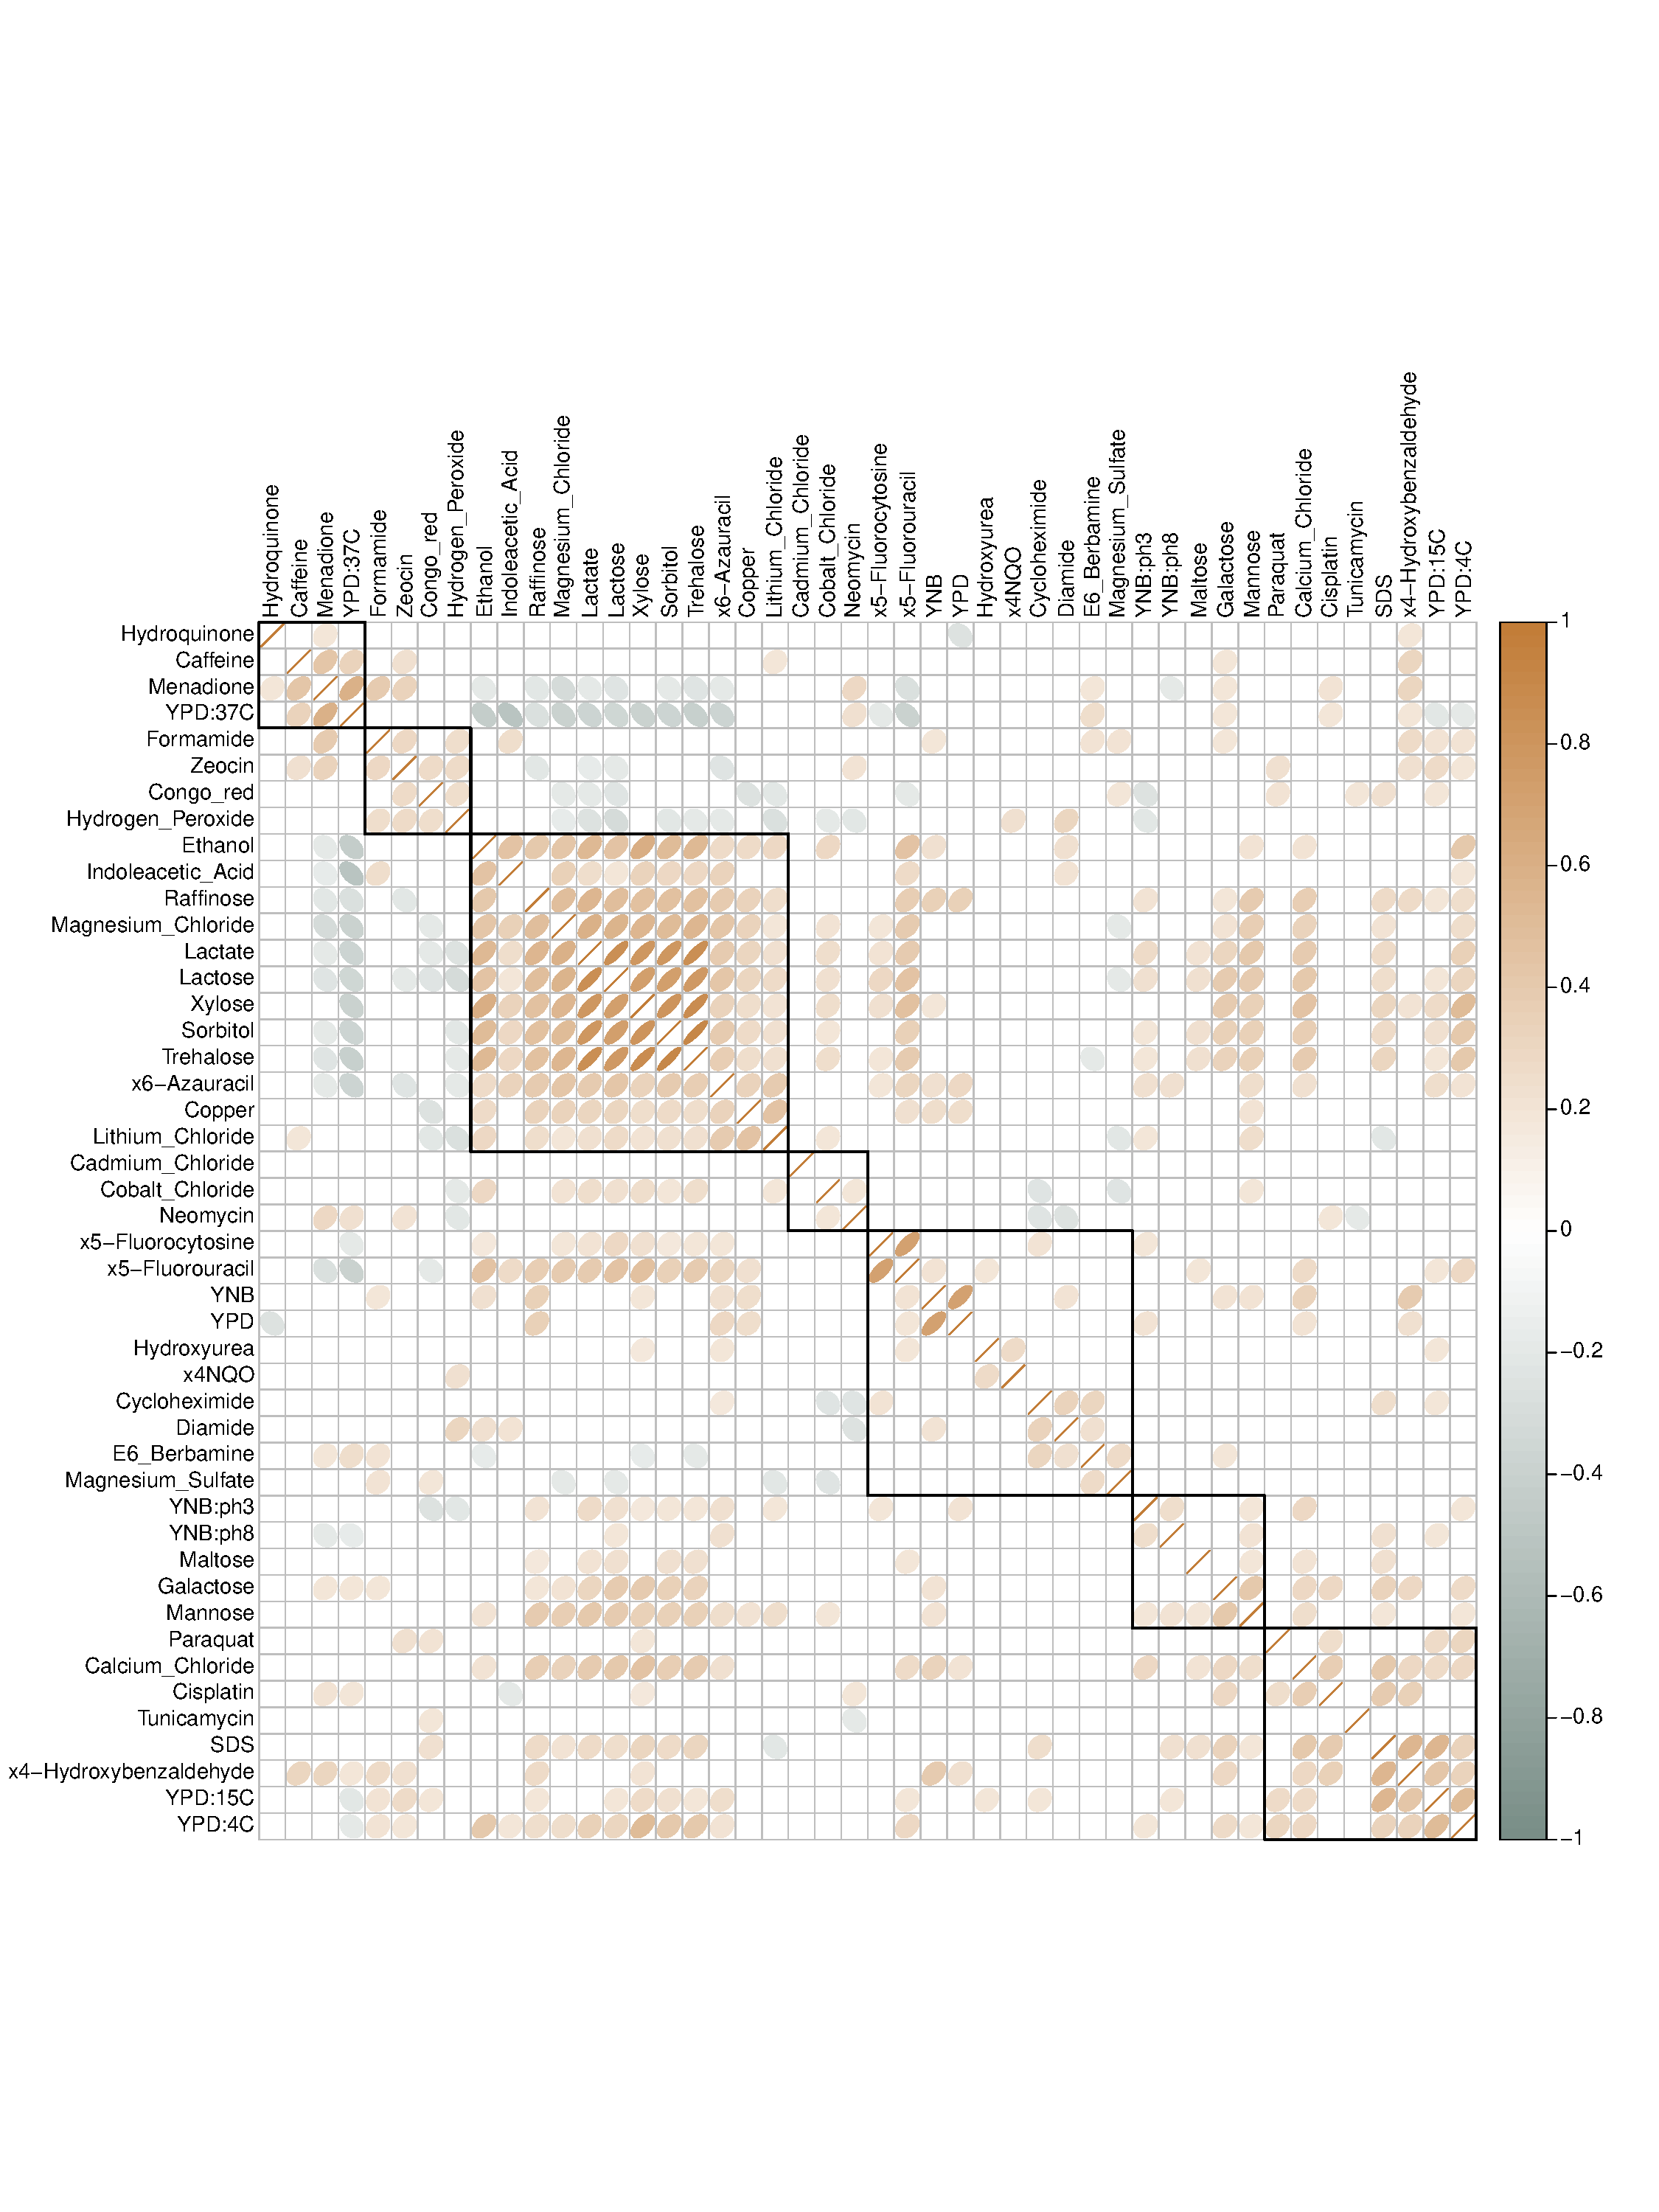
\includegraphics[trim = 0mm 80mm 10mm 80mm, clip, width=0.9\textwidth]{Chapter1/Figures/20170125_correlation_pheno_noNA.pdf}
	\caption[Pair-wise correlations of 46 growth traits in \emph{Saccharomyces cerevisiae}]{\textbf{Pair-wise correlations of 46 growth traits in \emph{Saccharomyces cerevisiae}.} For each trait pair, Spearman's rank correlation coefficient \(\rho\) and the p-values of the correlation were computed. The p-values were adjusted for multiple testing according to Benjamini and Hochberg's method \citep{Benjamini1995}. The strength and the direction of significant correlations (\(p < 0.05\)) are depicted above. Unsignificant correlations are left blank. The traits are clustered based on complete-linkage clustering of \((1-\rho)\) as distance measurement (R Package: \emph{corrplot}).}
 	\label{fig:traitcorrelations}
\end{figure}
 	
\begin{figure}[hbtp]
	\centering
	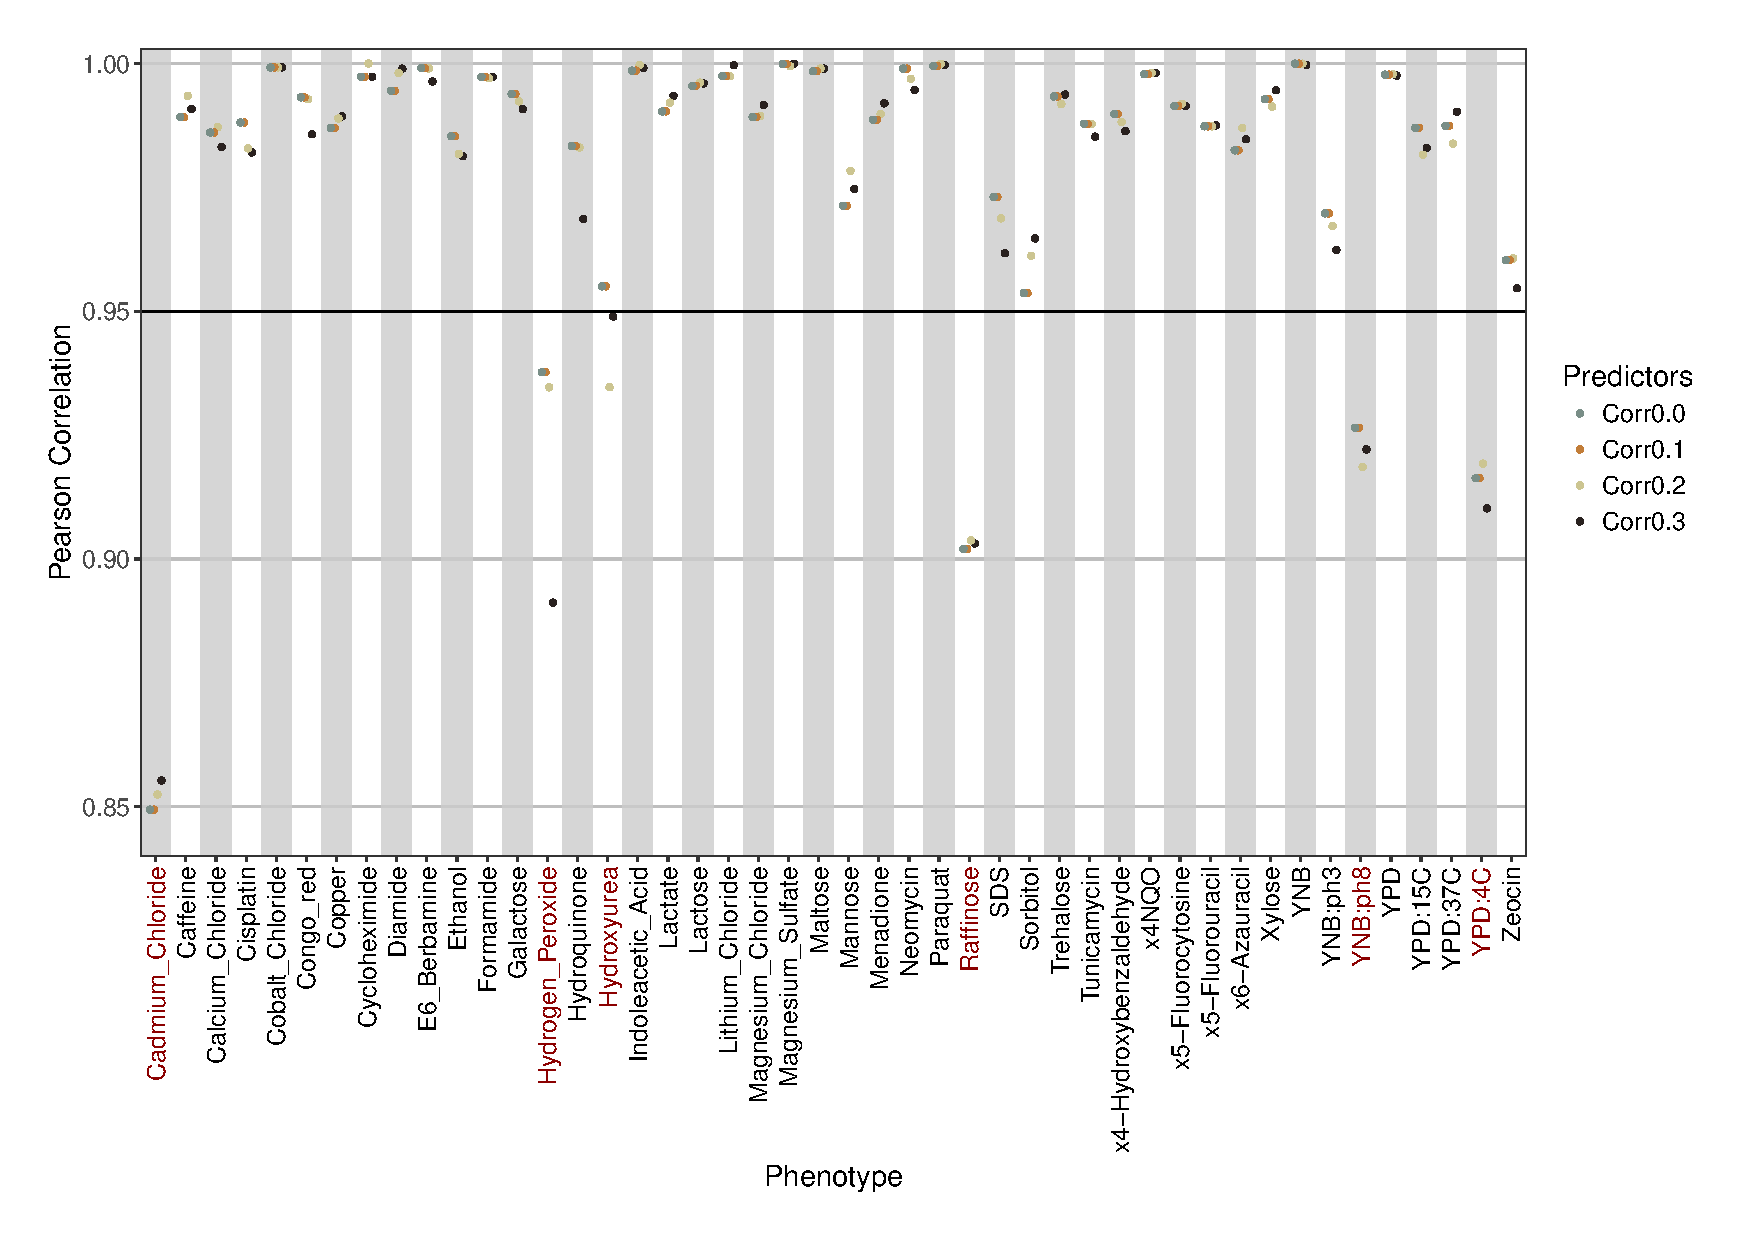
\includegraphics[trim = 0mm 0mm 0mm 0mm, clip, width=01\textwidth]{Chapter1/Figures/20170124_imputation_correlation_median_imputationvalue.pdf}
	\caption[Correlation between imputed and experimentally observed trait values]{\textbf{Correlation between imputed and experimentally observed trait values.} In the subset of 306 fully phenotyped samples, missing values were introduced and subsequently imputed via MICE. Different predictor sets were tested, differing in the predictors traits included. Sets were constructed based on different Spearman's rank correlation coefficient: traits were considered predictors if their correlation with the target trait was greater than a given threshold. For each predictor setup (\(\rho =\left\{0, 0.1, 0.2, 0.3\right\}\),   \(m=20\) multiple imputations and \(maxit=30\) iterations of MICE were conducted. The goodness of the imputation was evaluated by computing the correlation of the imputed values (averaged across iterations \(m\)) to the experimentally observed ones. Traits with at least one correlation greater than the 0.95 (black vertical line) were retained in the dataset. For traits labeled in red, the imputation was considered to be unreliable and the traits were excluded from further analyses (R Package: \emph{mice} \citep{vanBurren2011}).}
 	\label{fig:mice}
\end{figure}



\newpage
 \subsection{LiMMBo increases power in detecting genetic association in yeast}

\begin{itemize}
\item Assessing significance of association in yeast crosses via permutations \citep{Brehm2004, Ehrenreich2010}
\end{itemize} 
 
In order to test the performance of LiMMBo as a means for mtGWAS in a suitable set-up, i.e. in a cohort with related individuals, I conducted and compared an any effect mt-LMM-GWAS of 41 quantitative yeast traits to the results obtained in independent st-LMM-GWAS of the same traits. Figure~\ref{fig:GWAS-yeast} depicts the manhattan plot of both the st-LMM-GWAS p-values (adjusted for multiple testing by the effective number of tests \citep{Galwey2009}) and the mt-LMM-GWAS p-values. On several chromsomomes, mt-LMM-GWAS peaks (blue) are observed whereas no st-LMM-GWAS peaks (green) can be detected, demonstrating the increase in power by jointly modeling the traits. The heatmap below the mahattan plot shows the effect size estimates for each SNP for all 41 traits. Effect sizes were clustered based on their inner product across all SNPs. 
  \begin{figure}[hbtp]
	\centering
	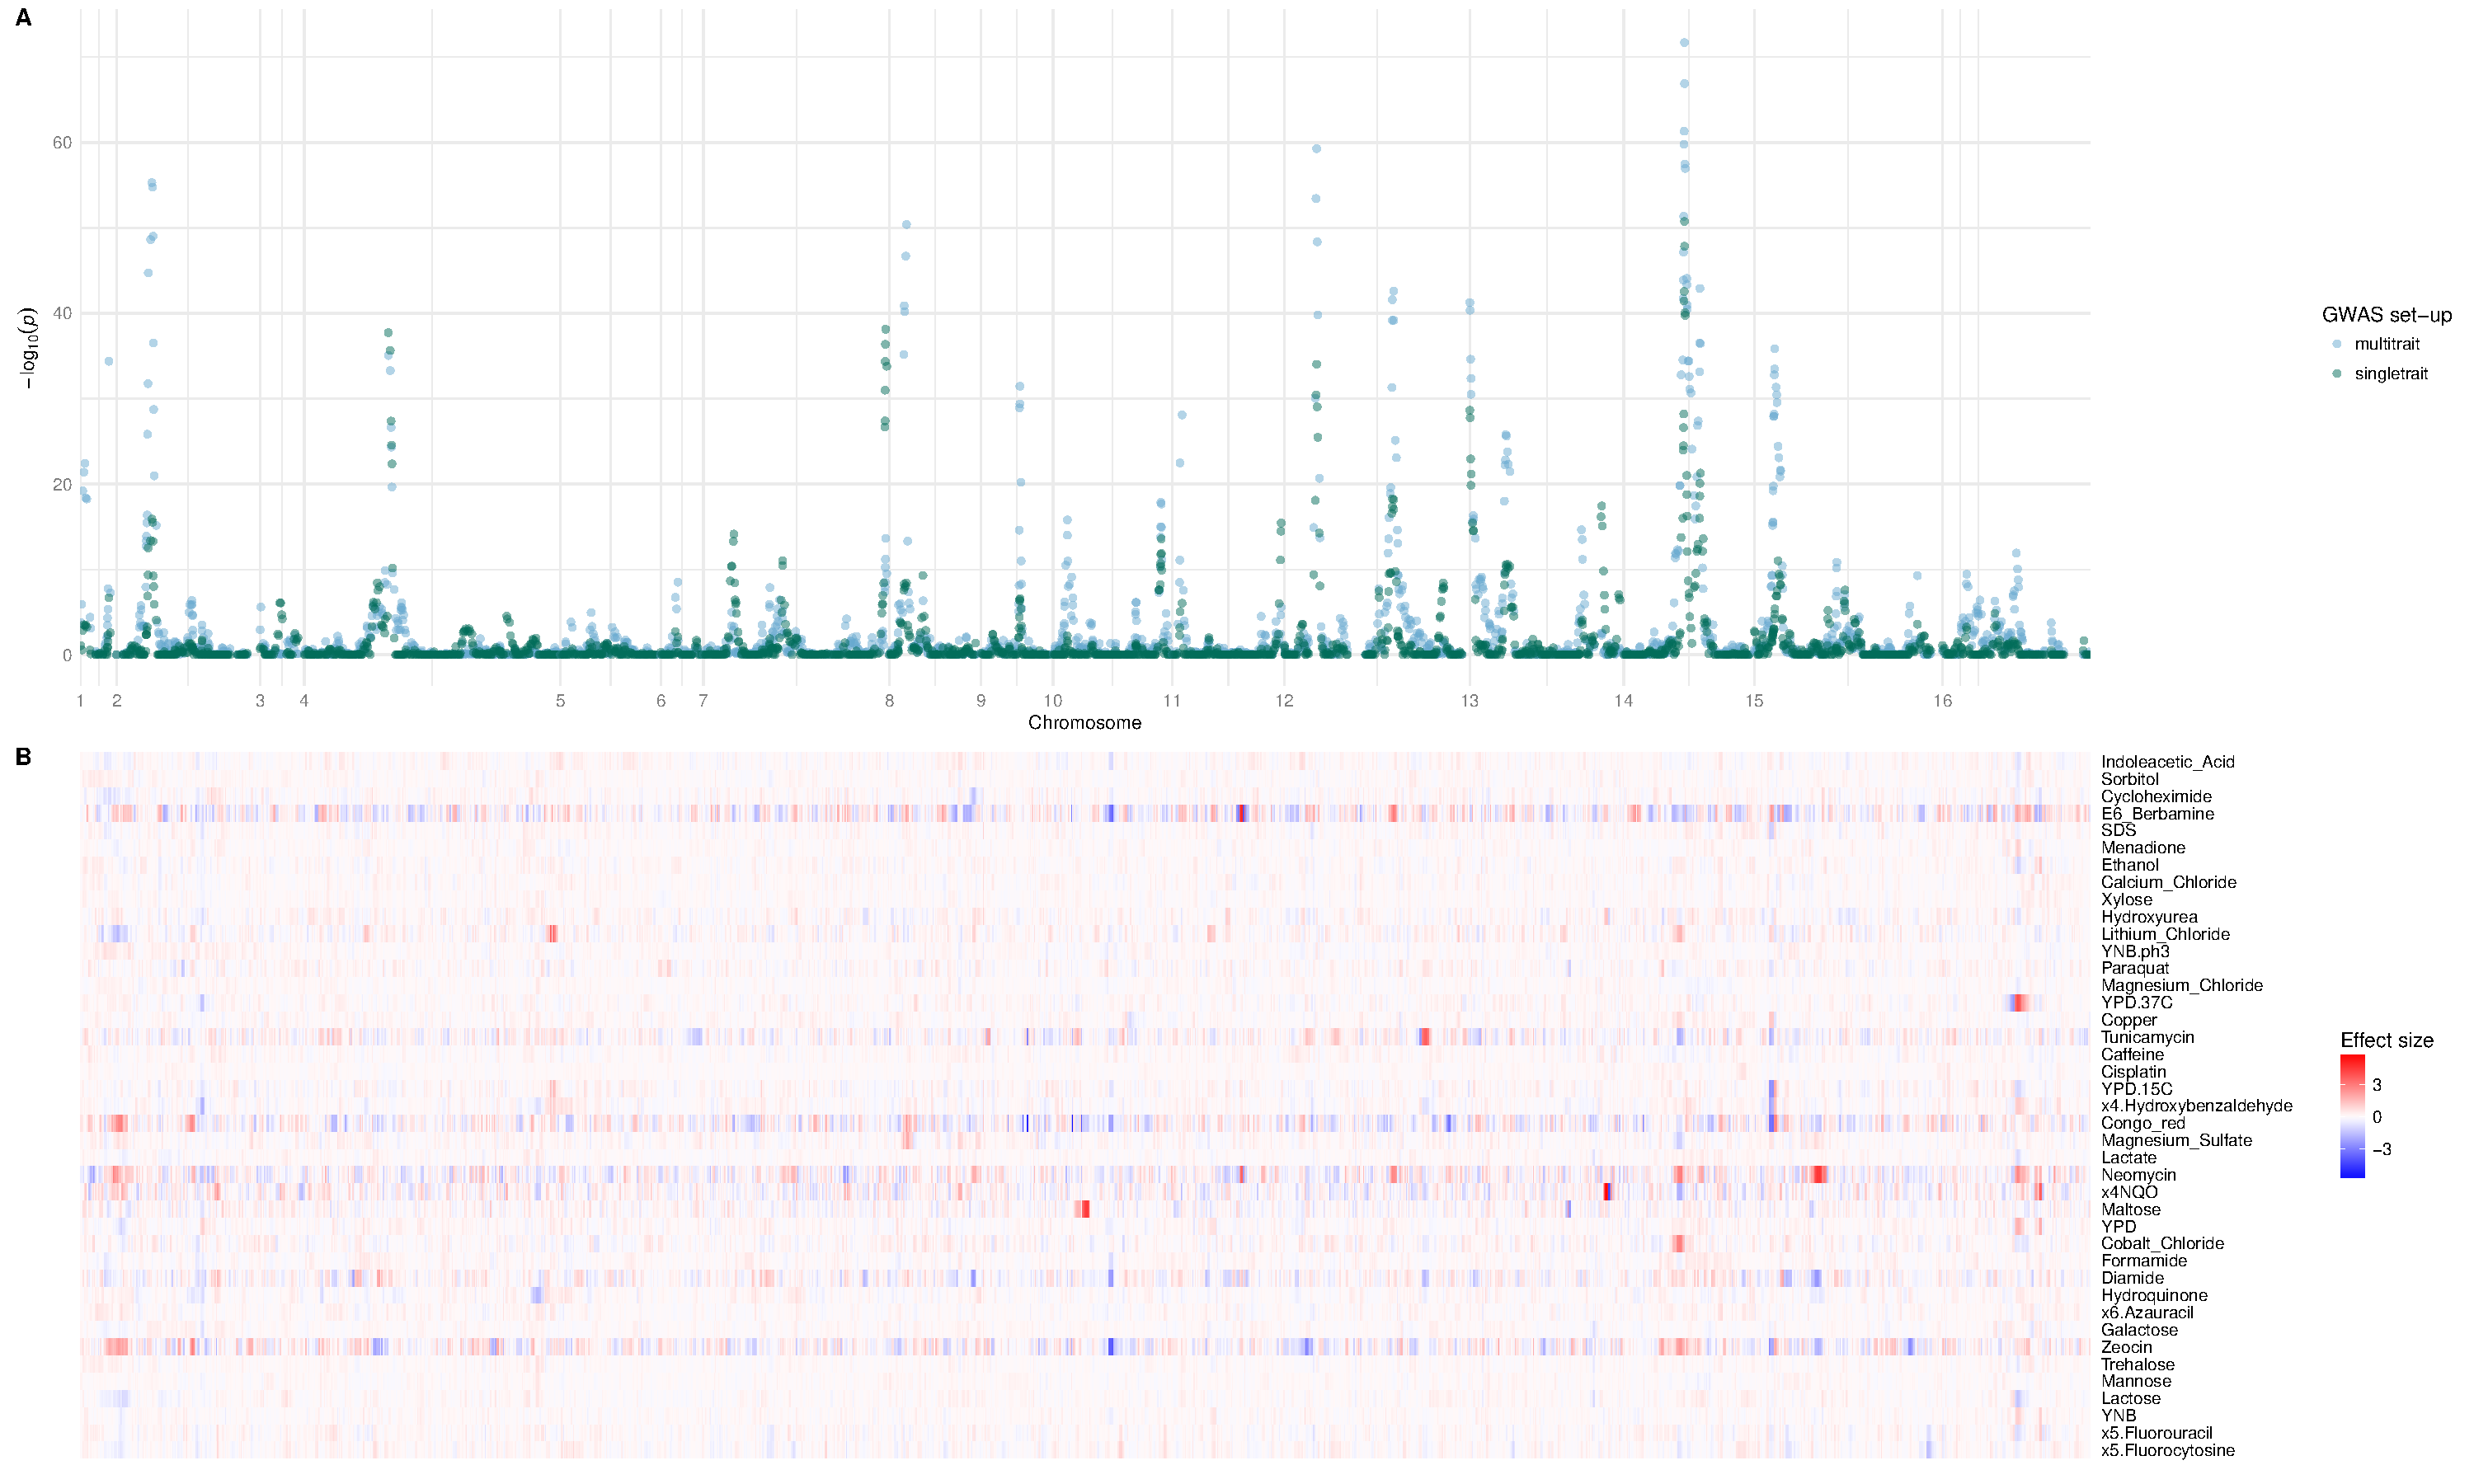
\includegraphics[trim = 0mm 0mm 0mm 0mm, clip, width=0.8\textwidth]{Chapter1/Figures/ManhattanEffectsizes.pdf}
	\caption[st-LMM-GWAS and any effect mt-LMM-GWAS of 41 quantitative traits in yeast]{\textbf{st-LMM-GWAS and any effect mt-LMM-GWAS of 41 quantitative traits in yeast.} (a) Manhattan plot of p-values from mt-LMM-GWAS (blue) and st-LMM-GWAS (green). Single-trait p-values are the minimum p-value per SNP for any of the 41 singletrait GWAS, adjusted for multiple testing by the effective number of test (\(T_{eff}=33\)). (b) Effect size estimates across the 41 jointly tested traits in the multitrait GWAS. Effect size estimate positions in the heatmap correspond the SNP positions in the manhattan plot.}
 	\label{fig:GWAS-yeast}
 	\end{figure}

